\section{Algoritmo Local Search}

\subsection{Solución}
La idea de un algorítmo de búsqueda local (o local search) es, a partir de una solución (no óptima) a un problema dado, trabajar sobre ella, realizar distintas operaciones y estrategias de modo tal de mejorarla e intentar acercarse lo más posible a una solución óptima. La distinción de éstos algoritmos está en que cada modificación a la solución original, nos genera una o un conjunto de soluciones al problema, siempre \"cercanas\" a la solución original. En éste sentido, definimos una \textit{vecindad} de soluciones, que está formada por éstas nuevas soluciones cercanas a la original. \\
En nuestro caso en particular, la idea es que, a partir de un grafo, hallemos un cojunto dominante de alguna forma (todos los nodos del grafo son, en efecto, un cojunto dominante. O bien también podemos usar la solución obtenida con el algoritmo greedy) y, a partir de ella, intentar construir, mediante estrategias y funciones creadas por nostros, una nueva solución, mejor o igual a la que nos proveyeron como base. \\
Es así que nos planteamos lo siguiente: ¿qué operaciones podemos realizar de forma tal que, a partir de un conjunto dominate, no necesariamente mínimo, podamos reducir la cardinalidad del conjunto y que continúe siendo dominante? Las posibilidades que encontramos fueron orientadas siempre a la posibilidad de reducir o, al menos mantener, la cantidad de nodos en el conjunto dominante. Es por eso que las estrategias que utilizamos en la búsqueda local son las siguientes: 

\begin{description}
\item[Reemplazar 2 nodos del Conjunto] dominante por uno que se encuentre dominado. Ésta es la forma más directa de reducir la cardinalidad del CD. La forma de seleccionar los nodos intercambiables la realizamos verificando si la unión de nodos vecinos de los dos nodos a quitar del conjunto está incluida en el conjunto formado por los vecinos del vértice a insertar en el CD. Ésta es la forma más sencilla de encontrar dichos nodos, ya que de otra forma, el costo de encontrar estos posibles reemplazos sería muy costoso. Además, existe la posibilidad de encontrar varios posibles candidatos, por lo que ideamos 3 funciones de comparación para ordenar éstas tuplas y, en cada caso, utilizar la más \"conveniente\" según dicha función. Luego, para el método GRASP, eligiremos una de éstas a partir de las pruebas realizadas.
\item[Eliminar 1 nodo del CD:] Para éste caso, analizamos si eliminando alguno de los nodos del CD, el mismo sigue dominando a todos los nodos del grafo. Para ello, nos fijamos si el conjunto de vecinos del nodo que queremos quitar, está incluido en la unión de todos los vecinos de los nodos del CD menos el nodo que queremos quitar. Si es así, quitando el nodo el conjunto seguirá siendo dominante. En éste caso, es claro que la cardinalidad disminuye.
\item[Reemplar 1 nodo del CD] por otro del conjunto dominado. La estrategia aplicada para encontrar los posibles candidatos es similar a la que utilizamos en la técnica del 2x1, es decir, nos fijamos los nodos que estén en el CD, y buscamos aquellos dominados cuyos conjunto de vecinos contenga a los vecinos del nodo quitado (no tienen que ser los mismos exactamente, podria tener mas vecinos). Es claro que ésta técnica no reduce la cardinalidad del conjunto, pero la utilizamos con la esperanza de que éste cambio de nodos nos modifique la solución parcial y, a partir de ésta, si podamos utilzar algunas de las técnicas anteriores. Es decir, lo que intentamos realizar con ésta procedimiento es que al cambiar por otro nodo con un número de nodos adyacentes posiblemente mayor, al agregarse nuevas aristas, podamos luego sí, en el próximo paso, reducir la cardinalidad del CD.
\end{description}

El algoritmo de búsqueda local intentará, a partir de una solución dada (en la primera iteración, será la solución que se le otorgue a la hora de invocarla), mejorarla a partir de alguna de las tres técnicas mencionadas anteriormen. Primero, intentará quitar 2 nodos del conjunto e ingresar uno. Si no puede, intentará con la siguiente estrategia, que es quitar uno del conjunto dominante. Si tampoco puede reducir la cardinalidad con ésta técnica, intentará reemplazar 1 nodo del CD por un nodo dominado, para así al menos, cambiar la solución. \\
Si alguna de éstas técnicas tuvo éxito, el algoritmo no probará con las siguientes, y a partir de la solución hallada, intentará volver a crear una nueva ejecutando todas las técnicas nuevamente para la nueva solución. Evidentemenete, llegará una solución para la que nuestro algoritmo no podrá llevar a cabo ninguna de las técnicas especificadas, y es ahí donde termina la búsqueda local, y nuestro algoritmo, dando como solución a la última encontrada, y que tendrá una cardinalidad igual o menor a la solución inicial. \\
A continuación, mostramos el pseudocódigo de nuestra algoritmo:  \\

\subsection{Pseudocódigo}
\begin{codebox}
\Procname{$\proc{MejorarSolucion}$ (\textbf{ConjuntoDominante} $cd$, \textbf{Comparator} $funcion$)}{cd}{Conjunto Dominante}
\li mejoroSolucion = true
\li	\textbf{hasta} mejoroSolucion no sea false: \Do
\li		mejoroSolucion = ElegirYEjecutarEstrategia(cd, funcion)
\End
\End
\li	\textbf{return} cd
\end{codebox}

\begin{codebox}
\Procname{$\proc{ElegirYEjecutarEstrategia}$ (\textbf{ConjuntoDominante} $cd$, \textbf{Comparator} $f$)}{res}{Boolean}
\li		\textbf{Si} es posible llevar a cabo la estrategia 2x1 con la funcion f: \Do
\li			devuelvo true
\End
\li		\textbf{Si} es posible llevar a cabo la estrategia quitar un nodo: \Do
\li			devuelvo true
\End
\li		\textbf{Si} es posible llevar a cabo la estrategia 1x1: \Do
\li			devuelvo true
\End
\li \textbf{return} false
\end{codebox}

\begin{codebox}
\Procname{$\proc{TryEstrategia2x1}$ (\textbf{ConjuntoDominante} $cd$, \textbf{Comparator} $f$)}{res}{Boolean}
\li		obtengo los posibles nodos intercambiables, ordenados por la funcion f
\li		\textbf{Si} existen posibles nodos intercambiables: \Do
\li			obtengo la primera tupla de nodos intercambiables
\li			intercambio los nodos de la tupla en el cd
\li			devuelvo true
\li		\textbf{sino} devuelvo false
\End
\li \textbf{return} false
\end{codebox}

\begin{codebox}
\Procname{$\proc{TryEstrategiaQuitarUno}$ (\textbf{ConjuntoDominante} $cd$, \textbf{Comparator} $f$)}{res}{Boolean}
\li		\textbf{para} cada vertice v del conjunto dominante: \Do
\li			quito el vertice v del cd
\li			\textbf{Si} el conjunto sigue siendo dominante: \Do
\li				devuelvo true
\End
\End
\li \textbf{return} false
\end{codebox}

\begin{codebox}
\Procname{$\proc{TryEstrategia1x1}$ (\textbf{ConjuntoDominante} $cd$, \textbf{Comparator} $f$)}{res}{Boolean}
\li		\textbf{para} cada vertice v del conjunto dominante: \Do
\li			\textbf{para} cada vertice d del conjunto dominado: \Do
\li				\textbf{si} no realize el intercambio v,d y los nodos son reemplazables: \Do
\li					intercambio los vertices en el cd
\li					devuelvo true
\End
\End
\End
\li \textbf{return} false
\end{codebox}

\subsection{Análisis de Complejidad}
Para todos los casos, se corre al menos k veces, y para cada una de esas k corridas, se utilizan 3 métodos para intentar hallar una nueva solucion:
\begin{description}
\item[2x1:] Se crea una cola de nodos, ordenados por una funcion f (pasada por parametro). Para ello, se recorren todos los posibles pares de nodos dominantes, y para cada par, se analiza si es posible reemplazarlo por un nodo del conjunto dominado. La complejidad de crear esta cola es de $O(n^2)$, siempre y cuando se considere que $n^2$ es mayor a m, siendo m la cantidad de vertices del conjunto dominado. Luego, para hacer el intercambio, se realizan operaciones en ArrayList, que son $O(n)$. Por lo que la complejidad de éste método es de $O(n^2)$.
\item[QuitarUno:] en éste caso, se recorren todos los nodos del conjunto dominante, y se pregunta si, quitando el nodo en cuestion, el conjunto continúa siendo dominante. Ésta método tiene una complejidad de $O(n x m)$, donde n es la cantidad de nodos del cd, y m es la cantidad de aristas de cada nodo.
 \item[UnOxUnO] ésta estrategia requiere de recorrer todos los vértices dominantes, y para cada uno de ellos, compararlo con todos los vértices dominados, y fijarme si puedo intercambiar éstos nodos (en cuestión, si tienen los mismos vecinos) de forma tal que el conjunto continue siendo dominante. Esta verificación es de complejidad $O(n x m)$, donde n es la cantidad de nodos del conjunto dominante, y m la cantidad de nodos del conjunto dominado.
\end{description}
 
 Es decir, que la complejidad en todos los casos, no es mayor a $O(n^2)$, ya que en todos los casos se analiza primero la opción de hacer el 2x1. Si puede, la complejidad será esa, y si no puede, seguirá con los otros métodos que, a rasgos generales, nunca superan ésta cota de $O(n^2)$. Por lo que la complejidad general del algoritmo es de \textbf{$O(n^2)$}.
 
 \subsection{Peor Caso}
 Es claro que, al ser una heurística, en muchos casos la solución obtenida por la búsqueda local (o local search) no es la óptima, pero de todas formas, se trata de soluciones "cercanas" a ella. En éste sentido, se dan cuando los nodos de la solución de la cual se parte la búsqueda loca, tienen muchas aristas conectadas entre si o a otros vértices ya dominados (los grados de los nodos son muy altos). Ésto hace que, por ejemplo, las estrategias elegidas no puedan intercambiar nodos, o quitar nodos de la solución de la que se parta y, sin embargo, en la práctica si exista una solución con menor cantidad de nodos. \\
En particular, hemos encontrado dos casos generales distintos: por un lado, aquellos en que el algorítmo de búsqueda local mejora la solución de la cual se parte pero, sin embargo, no llega a una solución óptima (calculada a partir del mismo grafo con el algoritmo exácto). Y por otro lado están aquellas instancias que, a partir de una solución, no pueden ser mejoradas por la búsqueda local, a pesar de haber una solución óptima y exacta con una menor cantidad de nodos. Éstos dos casos se pueden ver en los tests que hemos corrido en el jUnit, y que lamentablemente, no hemos podido correr para instancias de más de 25 nodos, ya que la solución exacta (que es de orden exponencial) no llega a terminarse y, por tanto, no podemos comparar los valores de la búsqueda local con los valores exactos. \\
\begin{center}
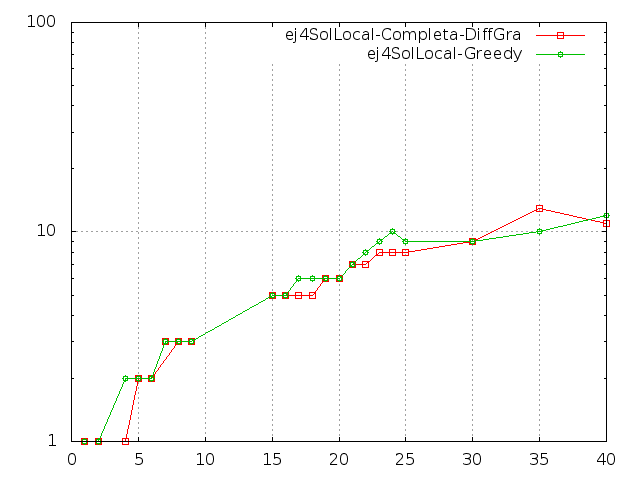
\includegraphics[width=12cm]{./graficos/comparacionSolucionPasadaLocal.png}
\end{center}
Éstos resultados, eran de esperarse, ya que se trata de una heurísitca y sólo en algunos casos partículares se consiguen los mismos resultados que en los algoritmos exáctos. La idea, entonces, es intentar de construir las mejores estrategias para poder llegar a un resultado lo más exacto posible, para instancias en que sea imposible (al menos hoy en día) correr el algoritmo exácto de orden exponencial. En éste caso particular, de la búsqueda local, seguramente haya muchas estrategias para mejorar o agregar, que nos aproximen a una solución un poco más exacta de la que encontramos hasta ahora, pero no pudimos dar con ellas.


\subsection{Tests y análisis}
En primer lugar, hemos hecho test para encontrar cuál de todas las funciones encuentra los nodos óptimos para el intercambio de nodos 2x1. En la teoría, todas analizan factores distintos, pero en la práctica, al ser muy pocos los nodos que pudimos intercambiar, las distintas funciones no han aportados cambios significativos en la cardinalidad de las soluciones. A lo sumo, ésta han diferido en 1 nodo, no más, y la que ha resultado más efectiva ha sido la de encontrar la diferencia de grados entre la tupla a quitar y el nodo a insertar. Es por eso que ésta función ha sido la que utilizamos para las pruebas restantes. \\
Una vez establecida qué función deberíamos utilizar para el 2x1, nos abocamos a testear el método de búsqueda local de acuerdo a la cantidad de nodos del grafo y el tiempo que le consume encontrar una solución. Vale aclarar que no tomamos en consideración el tiempo que nos consume encontrar una solución para darle a la búsqueda loca, ya que consideramos que ello no es parte de nuestro algoritmo. De ésta forma, podemos ver que nuestro algoritmo se comporta de forma polinómica en función del tiempo, como lo analizamos en la sección de complejidad. Es decir, mientras mayor cantidad de nodos tenga la solución que nos proveen, y más relacionados estén entre sí dichos nodos (es decir, a través de aristas hacia nodos del mismo conjunto o del conjunto de los dominados), mayor tiempo requerirá calcular nuestra solución. Además, y de forma conjunta con éste crecimiento, aumenta la cantidad de operaciones requeridas por el algortimo para finalizar cada iteración $k$, incremento que se ve directamente relacionado con el aumento de la cardinalidad de conjunto dominante. Ésto puede verse en el gráfico 1, de forma tal que a mayor cantidad de nodos que le pasamos a nuestra solución, mayor será el tiempo que le toma resolverlo, debido a que debe realizar más operaciones.

\begin{center}
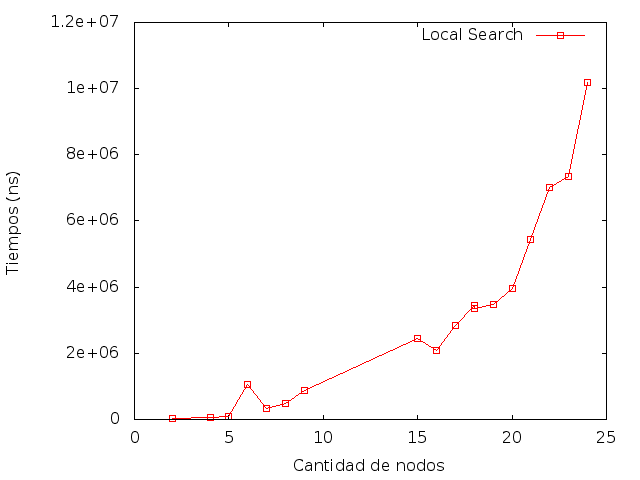
\includegraphics[width=13cm]{./graficos/tiempoLocalSearch.png}
\end{center}

Además, creemos conveniente probar / mostrar la mejoría que realiza nuestro algoritmo a las soluciones que se le dan. Para ello, comparamos la ejecución de la misma instancia para el algoritmo exacto, el algoritmo greedy y el algoritmo de solución local, y la calidad de la solución (la cardinalidad de las mismas), mostrando cómo mejoran las mismas de acuerdo a cada método. Es válido aclarar que en todas las corridas, hemos utilizado como instancia de entrada para el local search la solución  dada por el algoritmo greedy, por lo que en todos los casos, la cardinalidad de las soluciones de la búsqueda loca, será por lo menos, igual a la greedy y como máximo, si tuvimos suerte, igual a la exacta.

\begin{center}
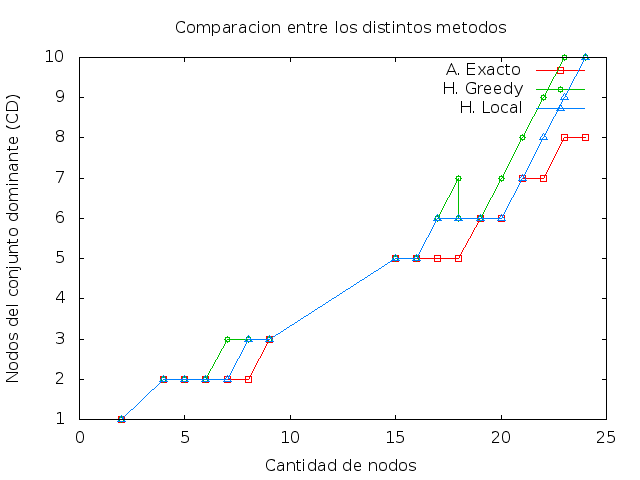
\includegraphics[width=13cm]{./graficos/local_comparacion_soluciones.png}
\end{center}
